\documentclass[../main.tex]{subfiles}
\graphicspath{{figures/}{../figures/}}

\begin{document}
  % \todo[color=green!30]{完成问题二模型的建立(sections/q2\_build)}
  \noindent\textbf{Step 1 证明板凳龙首次发生碰撞一定是第 1 节板凳或第 2 节板凳与其他板凳碰撞}
  \par 假设在第$t$秒时,板凳龙首次发生碰撞,且第$i(3\leq i\leq 223)$节板凳与第$j(2\leq j<i)$板凳发生碰撞。由于各节板凳把手中心沿等距螺线运动,又设第$j-1$节板凳的前把手中心运动到第$i$节板凳前把手中心在第t秒时的位置的时刻为$t_1$秒。由于运动的先后顺序,显然$t_1<t$。
  \par 通过给定条件可知,$1\leq j-1\leq i-1$.当j - 1 = 1时,结论成立。当j不等于1,即$2\leq j-1\leq i-1$时,由于除第一节板凳外,其余板凳长度均相同且运动轨迹一致,因此若在第$t_{1}$秒,第$j - 1$节板凳前后把手中心位置与第j节板凳在第t秒的前后把手中心位置不同,那么在第$t_{1}$秒时,第$j - 1$节板凳必然会与其他板凳发生碰撞,这与第t秒首次碰撞的假设矛盾。
  \par 由此可得,在第$t_1$秒时第$m$节板凳前后把手中心的位置一定与在第$t$秒时第$m+1$节板凳前后把手中心的位置相同,其中$m=j-1,j-2,\cdots,2$.有
  \begin{align}\label{1.........18}
  P_m\left( t \right) =P_{m-1}\left( t_1 \right) ,m=2,3,\cdots ,j.
  \end{align}
  \par 即第$j - 1$节板凳在第$t_{1}$秒和第i节板凳在第t秒位置相同,第$i - 1$节板凳在第$t_{1}$秒和第i节板凳在第t秒位置也相同,由假设可知第$j - 1$节和第$i - 1$节板凳在第$t_{1}$秒会碰撞,与板凳龙在第t秒首次碰撞矛盾。所以假设不成立,因此板凳龙首次发生碰撞一定是第1节板凳或第2节板凳与其他板凳碰撞。
 
  \noindent\textbf{Step 2 计算各节板凳四个顶点的坐标}
  \par 当第$i(i=1,2,\cdots,223)$节板凳后把手刚盘入螺线(即后把手恰好在初始位置)时,记离原点较远且离$P_i$较近的顶点为$A_i$,再按顺时针方向分别记其余顶点为$B_i,C_i,D_i$,并记$B_iC_i$和$A_iD_i$的中点分别为$E_i,F_i$,如下图所示。
  \begin{figure}[H]
     \centering
     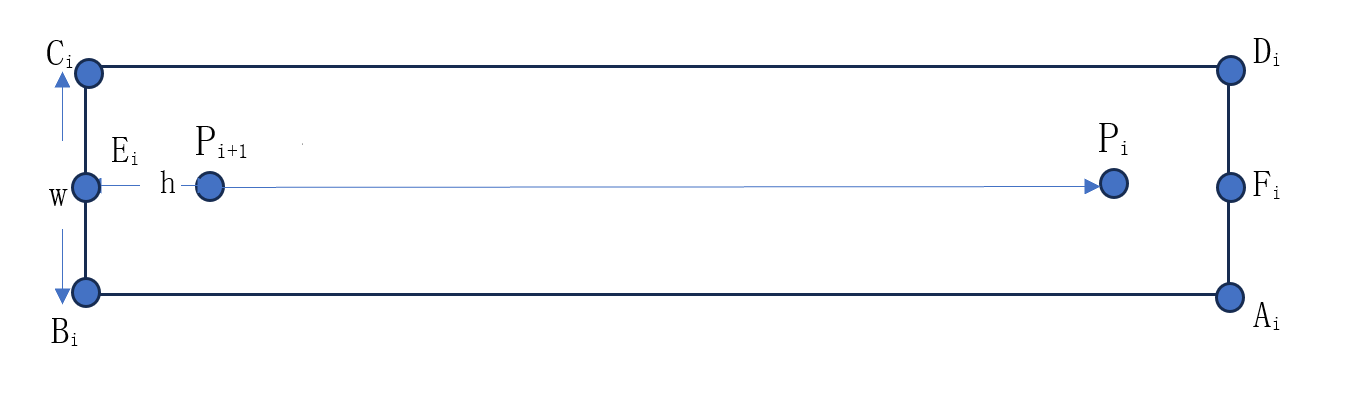
\includegraphics[width=.6\textwidth]{tupian}
     \caption{板凳顶点示意图}
     \label{fig:circuit-diagram}
 \end{figure}
 \par 设第$i(i=1,2,\cdots,223)$节板凳后把手中心在第$t$秒的直角坐标为$(x_0(t),y_0(t))$,
 $(x_i(t),y_i(t))$.设所有板凳的板宽均为$w$,板凳把手中心离最近的板头距离为$h$,则由条件可知$w=0.3m,h=0.275m$.
 
 
  \par 记$A_i,B_i,C_i,D_i$在第$t$秒时的位置分别为$A_i(t),B_i(t),C_i(t),D_i(t)$,其直角坐标分别为$(x_{A_i}(t),y_{A_i}(t)),(x_{B_i}(t),y_{B_i}(t)),(x_{C_i}(t),y_{C_i}(t)),(x_{D_i}(t),y_{D_i}(t))$,因此
  \begin{gather}
  \overrightarrow{P_{i+1}\left( t \right) P_i\left( t \right) }=\left( x_i\left( t \right) -x_{i+1}\left( t \right) ,y_i\left( t \right) -y_{i+1}\left( t \right) \right) \label{problem-2.1}
 \\
 \left| \overrightarrow{A_i\left( t \right) D_i\left( t \right) } \right|=\left| \overrightarrow{B_i\left( t \right) C_i\left( t \right) } \right|=w\label{problem-2.3}
 \end{gather}
 \par 于是根据向量垂直坐标变换公式可得,对$\forall i\in {0,1,2,\cdots,222}$,都有
 \begin{gather}
 \overrightarrow{A_i\left( t \right) D_i\left( t \right) }=\overrightarrow{B_i\left( t \right) C_i\left( t \right) }=\left( -\left[ y_i\left( t \right) -y_{i+1}\left( t \right) \right] ,x_i\left( t \right) -x_{i+1}\left( t \right) \right) \label{problem-2.2}
 \end{gather}
  \par 对于$B_iC_i$和$A_iD_i$的中点$E_i,F_i$,设它们在第$t$秒时的位置分别为$E_i(t),F_i(t)$,直角坐标分别为
  \begin{align}
     E_i(t)=(x_{E_i}(t),y_{E_i}(t)),\label{1.........20}
     \\
     F_i(t)=(x_{F_i}(t),y_{F_i}(t)).\label{1.........21}
     \end{align}
     从而
     \begin{gather}
     \overrightarrow{P_{i+1}\left( t \right) E_i\left( t \right) }=\left( x_{E_i}\left( t \right) -x_{i+1}\left( t \right) ,y_{E_i}\left( t \right) -x_{i+1}\left( t \right) \right) ,\label{problem-2.4}
     \\
     \overrightarrow{P_i\left( t \right) F_i\left( t \right) }=\left( x_{F_i}\left( t \right) -x_i\left( t \right) ,y_{F_i}\left( t \right) -x_i\left( t \right) \right) ,\label{problem-2.5}
     \\
     \left| \overrightarrow{P_{i+1}\left( t \right) E_i\left( t \right) } \right|=\left| \overrightarrow{P_i\left( t \right) F_i\left( t \right) } \right|=h.\label{problem-2.6}
     \\
     \overrightarrow{E_i\left( t \right) B_i\left( t \right) }=\left( x_{B_i}\left( t \right) -x_{E_i}\left( t \right) ,y_{B_i}\left( t \right) -y_{E_i}\left( t \right) \right) ,\label{problem-2..1}
     \\
     \overrightarrow{E_i\left( t \right) C_i\left( t \right) }=\left( x_{C_i}\left( t \right) -x_{E_i}\left( t \right) ,y_{C_i}\left( t \right) -y_{E_i}\left( t \right) \right) ,\label{problem-2..2}
     \\
     \overrightarrow{F_i\left( t \right) A_i\left( t \right) }=\left( x_{A_i}\left( t \right) -x_{F_i}\left( t \right) ,y_{A_i}\left( t \right) -y_{F_i}\left( t \right) \right) ,\label{problem-2..3}
     \\
     \overrightarrow{F_i\left( t \right) D_i\left( t \right) }=\left( x_{D_i}\left( t \right) -x_{F_i}\left( t \right) ,y_{D_i}\left( t \right) -y_{F_i}\left( t \right) \right) .\label{problem-2..4}
     \end{gather}
     由$E_i,P_i,P_{i+1},F_i$共线可得
     \begin{gather}
     \overrightarrow{P_{i+1}\left( t \right) E_i\left( t \right) }=-\frac{\overrightarrow{P_{i+1}\left( t \right) P_i\left( t \right) }}{\left| \overrightarrow{P_{i+1}\left( t \right) P_i\left( t \right) } \right|}\cdot \left| \overrightarrow{P_{i+1}\left( t \right) E_i\left( t \right) } \right|,\label{problem-2.7}
     \\
     \overrightarrow{P_i\left( t \right) F_i\left( t \right) }=\frac{\overrightarrow{P_{i+1}\left( t \right) P_i\left( t \right) }}{\left| \overrightarrow{P_{i+1}\left( t \right) P_i\left( t \right) } \right|}\cdot \left| \overrightarrow{P_{i+1}\left( t \right) E_i\left( t \right) } \right|.\label{problem-2.8}
     \end{gather}
     联立\eqref{problem-2.1}\eqref{problem-2.4}\eqref{problem-2.5}\eqref{problem-2.6}\eqref{problem-2.7}\eqref{problem-2.8}式可得
     \begin{gather}
     \begin{cases}
     x_{E_i}\left( t \right) =x_{i+1}\left( t \right) -\frac{h}{l_{i+1}}\left( x_i\left( t \right) -x_{i+1}\left( t \right) \right)\\
     y_{E_i}\left( t \right) =y_{i+1}\left( t \right) -\frac{h}{l_{i+1}}\left( y_i\left( t \right) -y_{i+1}\left( t \right) \right)\\
     \end{cases},\label{problem-2.9}
     \\
     \begin{cases}
     x_{F_i}\left( t \right) =x_i\left( t \right) +\frac{h}{l_{i+1}}\left( x_i\left( t \right) -x_{i+1}\left( t \right) \right)\\
     y_{F_i}\left( t \right) =y_i\left( t \right) +\frac{h}{l_{i+1}}\left( y_i\left( t \right) -y_{i+1}\left( t \right) \right)\\
     \end{cases}.\label{problem-2.10}
     \end{gather}
     又由$E_i$是$B_i,C_{i}$的中点和$F_i$是$A_i,D_i$的中点可得
     \begin{gather}
     \overrightarrow{E_i\left( t \right) B_i\left( t \right) }=-\frac{\overrightarrow{B_i\left( t \right) C_i\left( t \right) }}{2},\label{problem-2.11}
     \\
     \overrightarrow{E_i\left( t \right) C_i\left( t \right) }=\frac{\overrightarrow{B_i\left( t \right) C_i\left( t \right) }}{2},\label{problem-2.12}
     \\
     \overrightarrow{F_i\left( t \right) A_i\left( t \right) }=-\frac{\overrightarrow{A_i\left( t \right) D_i\left( t \right) }}{2},\label{problem-2.13}
     \\
     \overrightarrow{F_i\left( t \right) D_i\left( t \right) }=\frac{\overrightarrow{A_i\left( t \right) D_i\left( t \right) }}{2}.   \label{problem-2.14} 
     \end{gather}
     因此联立\eqref{problem-2.2}\eqref{problem-2.3}\eqref{problem-2..1}\eqref{problem-2..2}\eqref{problem-2..3}\eqref{problem-2..4}\eqref{problem-2.9}\eqref{problem-2.10}\eqref{problem-2.11}\eqref{problem-2.12}\eqref{problem-2.13}式,解得板凳的四个顶点坐标。
     \begin{gather}
     \begin{cases}
     x_{A_i}\left( t \right) =x_i\left( t \right) +\frac{h}{l_{i+1}}\left( x_i\left( t \right) -x_{i+1}\left( t \right) \right) +\frac{y_i\left( t \right) -y_{i+1}\left( t \right)}{2}\\ \label{1.........24}
     y_{A_i}\left( t \right) =y_i\left( t \right) +\frac{h}{l_{i+1}}\left( y_i\left( t \right) -y_{i+1}\left( t \right) \right) -\frac{x_i\left( t \right) -x_{i+1}\left( t \right)}{2}\\ 
     \end{cases},
     \\
     \begin{cases}
     x_{B_i}\left( t \right) =x_{i+1}\left( t \right) -\frac{h}{l_{i+1}}\left( x_i\left( t \right) -x_{i+1}\left( t \right) \right) +\frac{y_i\left( t \right) -y_{i+1}\left( t \right)}{2}\\ \label{1.........26}
     y_{B_i}\left( t \right) =y_{i+1}\left( t \right) -\frac{h}{l_{i+1}}\left( y_i\left( t \right) -y_{i+1}\left( t \right) \right) -\frac{x_i\left( t \right) -x_{i+1}\left( t \right)}{2}\\ 
     \end{cases},
     \\
     \begin{cases}
     x_{C_i}\left( t \right) =x_{i+1}\left( t \right) -\frac{h}{l_{i+1}}\left( x_i\left( t \right) -x_{i+1}\left( t \right) \right) -\frac{y_i\left( t \right) -y_{i+1}\left( t \right)}{2}\\ \label{1.........28}
     y_{C_i}\left( t \right) =y_{i+1}\left( t \right) -\frac{h}{l_{i+1}}\left( y_i\left( t \right) -y_{i+1}\left( t \right) \right) +\frac{x_i\left( t \right) -x_{i+1}\left( t \right)}{2}\\ 
     \end{cases},
     \\
     \begin{cases}
     x_{D_i}\left( t \right) =x_i\left( t \right) +\frac{h}{l_{i+1}}\left( x_i\left( t \right) -x_{i+1}\left( t \right) \right) -\frac{y_i\left( t \right) -y_{i+1}\left( t \right)}{2}\\   \label{1.........30}
     y_{D_i}\left( t \right) =y_i\left( t \right) +\frac{h}{l_{i+1}}\left( y_i\left( t \right) -y_{i+1}\left( t \right) \right) +\frac{x_i\left( t \right) -x_{i+1}\left( t \right)}{2}\\   
     \end{cases}.
     \end{gather}
     \noindent\textbf{Step 2 碰撞判断模型}
 \par 确定板凳龙盘入发生碰撞前的终止时刻,可以先求解板凳龙何时发生碰撞,并将发生碰撞问题转化为板凳对应的边界有交点的问题。对于任意大于0的时刻 \(t\) ,板凳龙在第 \(t\) 秒发生碰撞的充分必要条件是:存在 \(s\) 和 \(k\) ,且 \(s, k \in \{1, 2, \cdots, 223\}\) ,使得在第 \(t\) 秒时,由 \(A_s(t)\) 、 \(B_s(t)\) 、 \(C_s(t)\) 、 \(D_s(t)\) 所确定的矩形与 \(A_k(t)\) 、 \(B_k(t)\) 、 \(C_k(t)\) 、 \(D_k(t)\) 所确定的矩形存在交点,这意味着对应的两节板凳发生了碰撞。因此,我们的核心任务就转变为在每一秒,对所有可能的 \(i\) 和 \(j\) (\(i, j \in \{1, 2, \cdots, 223\}\) ,$i\ne j$),判断矩形 \(A_i(t)B_i(t)C_i(t)D_i(t)\) 和矩形 \(A_j(t)B_j(t)C_j(t)D_j(t)\) 是否有交点。
 \par 为了有效判断两个矩形是否相交,我们借助向量叉乘的性质(详见\href{https://zhuanlan.zhihu.com/p/644689588}{几何算法:判断两条线段是否相交})来设计判定算法。从矩形 \(A_i(t)B_i(t)C_i(t)D_i(t)\) 中任选一条边,记为 \(X_1(t)Y_1(t)\) ,同时从矩形 \(A_j(t)B_j(t)C_j(t)D_j(t)\) 中选取一条边,记为 \(X_2(t)Y_2(t)\) 。
 \begin{align}\label{1.........32}
     \begin{cases}
     \text{若}\left( \overrightarrow{X_1\left( t \right) Y_1\left( t \right) }\times \overrightarrow{X_1\left( t \right) X_2\left( t \right) } \right) \cdot \left( \overrightarrow{X_1\left( t \right) Y_1\left( t \right) }\times \overrightarrow{X_1\left( t \right) Y_2\left( t \right) } \right) >0,\text{则判定}\overrightarrow{X_1\left( t \right) Y_1\left( t \right) },
     \\\overrightarrow{X_2\left( t \right) Y_2\left( t \right) }\text{相交}.\\
     \text{若}\left( \overrightarrow{X_1\left( t \right) Y_1\left( t \right) }\times \overrightarrow{X_1\left( t \right) X_2\left( t \right) } \right) \cdot \left( \overrightarrow{X_1\left( t \right) Y_1\left( t \right) }\times \overrightarrow{X_1\left( t \right) Y_2\left( t \right) } \right) \leqslant 0,\text{则判定}\overrightarrow{X_1\left( t \right) Y_1\left( t \right) },
     \\\overrightarrow{X_2\left( t \right) Y_2\left( t \right) }\text{不相交}.\\
     \end{cases}
     \end{align}
     \par 为了准确判断矩形 \(A_i(t)B_i(t)C_i(t)D_i(t)\) 和矩形 \(A_j(t)B_j(t)C_j(t)D_j(t)\) 是否相交,需要将矩形 \(A_i(t)B_i(t)C_i(t)D_i(t)\) 的四条边分别与矩形 \(A_j(t)B_j(t)C_j(t)D_j(t)\) 的四条边按照上述规则进行逐一判断。只有当所有边对判断的结果都显示不相交时,才能确定这两个矩形不存在交点,即两节板凳不发生碰撞;只要存在一组边对判断结果为相交,就可以认定这两个矩形存在交点,即两节板凳发生碰撞。
  \\\noindent\textbf{Step 3 模型求解方法}
 \par 首先,我们将初始步长$\varDelta t_0$ 设为 1 秒.然后,从 \(t = 0\) 开始,以步长 $\varDelta t_0$ 进行遍历。在每一个时间点 \(t\) ,对于所有的 \(i \in \{1, 2, \cdots, 223\}\) ,将矩形 \(A_{i}(t)B_{i}(t)C_{i}(t)D_{i}(t)\) 和矩形 \(A_{1}(t)B_{1}(t)C_{1}(t)D_{1}(t)\) 或矩形 \(A_{i}(t)B_{i}(t)C_{i}(t)D_{i}(t)\)分别代入Step 2中的碰撞判断模型判断是否相交。若在当前步长下遍历完所有时间点都未发现碰撞,则对步长进行调整,增加步长时间,然后继续上述步骤。如果在某一时刻 \(t\) ,发现存在相交情况,记录此时的时间 \(t\),确定碰撞时间范围,缩短时间步长为原来的\(\frac{1}{100}\)或\(\frac{1}{10}\) ,在碰撞时间范围内继续进行循环判断。最后,不断调整时间和步长,直到找到舞龙队发生碰撞前的时刻。
  \\\noindent\textbf{Step 4 位置与速度}
 \par 将Step 3求得的舞龙队发生碰撞前的时刻代入问题一的模型当中,利用Python求解得到此时板凳龙各把手的位置直角坐标和速度。
 

\end{document}